 %!TEX TS-program = xelatex

%	Author: Dmitry Rodin (d.rod1n1721@gmail.com)
%	

%	Основной документ
\documentclass[a4paper, 14pt]{extarticle}	%	14-й шрифт дл текста

%	Преамбула для оформления файла Latex
%	Преамбула

%	Шрифты

%	Гиперссылки

%	Отступы по ГОСТ

%	Секции без номеров(ВВЕДЕНИЕ, ЗАКЛЮЧЕНИЕ, СОКРАЩЕНИЯ ПРИНЯТЫЕ В ТЕКСТЕ....)
\newcommand{\anonsection}[1]{
	\phantomsection % Корректный переход по ссылкам в содержании
	\paragraph{\centerline{{#1}}\vspace{1.5em}}
	\addcontentsline{toc}{section}{\uppercase{#1}}
}

%	Библиография
\makeatletter
\renewenvironment{thebibliography}[1]
{\section*{\refname}
	\list{\@biblabel{\@arabic\c@enumiv}}
	{\settowidth\labelwidth{\@biblabel{#1}}
		\leftmargin\labelsep
		\itemindent 16.7mm
		\@openbib@code
		\usecounter{enumiv}
		\let\p@enumiv\@empty
		\renewcommand\theenumiv{\@arabic\c@enumiv}
	}
	\setlength{\itemsep}{0pt}
}
\makeatother

%	Начало документа
\begin{document}
	
	%	Содержание
	\tableofcontents
	\clearpage
	
	%	Сокращения, принятые в тексте
	\anonsection{СОКРАЩЕНИЯ, ПРИНЯТЫЕ В ТЕКСТЕ}

\begin{tabular}{ l l  }
	БСК & блок силовой коммутации \\
	БУК	&	блок усиления и коммутации\\
	БЦВМ &	бортовая цифровая вычислительная машина\\
	БЭ &		блок электроники\\
	ВА &		возвращаемый аппарат\\
	ДДУ &		дискретный датчик угла\\
	ИТ	&	источник тока\\
	НС	&	наблюдатель состояния\\
	ОУ	&	объект управления\\
	ПТДУ &	посадочная твердотопливная двигательная установка\\
	ПТК НП &	пилотируемый транспортный корабль нового поколения \\
	ПУ	&	посадочное устройство\\
	РДТТ	&	ракетный двигатель твердого топлива\\
	РМ	&	рулевая машинка\\
	РП	&	рулевой привод\\
	РПУ	&	релейное пороговое устройство\\
	РС	&	регулятор состояния\\
	СУ	&	система управления\\
	СУБ	&	сопловые управляемые блоки\\
	ТП	&	телеметрический потенциометр\\
	ТРТ	&	твердое ракетное топливо\\
	УПК	&	устройство преобразования кода Грея в двоичный код\\
	УСДК &	устройство сравнения двоичных кодов\\
	ЭД	&	электродвигатель\\
	ЭП	&	электромеханический привод\\
	
\end{tabular}

\clearpage
	
	%	Введение
	%	Введение
\anonsection{Введение}

Целью данного курсового проекта является синтез алгоритма наведения и стабилизации центра масс возвращаемого аппарата. Разработка алгоритмов и программного обеспечения математического моделирования замкнутой системы управления в MatLab. Проведение сравнительного анализа результатов моделирования.


Под синтезом системы автоматического управления понимается направленный расчет, имеющий конечной целью отыскание рациональной структуры системы и установление оптимальных величин параметров ее отдельных звеньев. 

Синтез можно трактовать как инженерную задачу, сводящуюся к такому построению системы, при котором обеспечивается выполнение технических требований к ней. Подразумевается, что из многих возможных решений инженер, проектирующий систему, будет выбирать те, которые являются оптимальными с точки зрения существующих конкретных условий и требований к габаритам, весу, простоте, надежности и т. п.

При инженерном синтезе системы автоматического управления необходимо обеспечить, во-первых, требуемую точность и, во-вторых, приемлемый характер переходных процессов.

Обеспечение приемлемых переходных процессов оказывается почти всегда более трудным вследствие большого числа варьируемых параметров и многозначности решения задачи демпфирования системы. Поэтому существующие инженерные методы часто ограничиваются решением только второй задачи, так как обеспечение требуемой точности может быть достаточно просто сделано на основании использования существующих критериев точности и совершенствования их практически не требуется.

В настоящее время для целей синтеза систем автоматического управления широко используются вычислительные машины, позволяющие производить полное или частичное моделирование проектируемой системы
\clearpage
	
	%	Техническое задание на разработку СУ ПТДУ
	%	Требования технического задания на разработку СУ ПТДУ
\anonsection{ОСНОВНАЯ ЧАСТЬ}
\section{Требования технического задания на разработку СУ ПТДУ}

\begin{enumerate}
	\item Рассматривается схема газосвязанной ПТДУ с регулированием тяги
	
	\item Основные потребные параметры ПТДУ определяются значениями
	\begin{itemize}
		\item Диапазон суммарной тяги $R_{\sum} = 9.0 - 22.0$ тс, при этом предполагается возможность реализации управления тягой по заданным алгоритмам в зависимости от реализованных условий посадки, обусловленных разбросом параметров атмосферы, аэродинамических, массовых, инерционных, центровочных характеристик возвращаемого аппарат, параметров, траектории и др
		\item Суммарный импульс тяги по осям всех сопел $I_{\sum} = 260 \text{тс}*\text{c}$
		\item Максимальное время работы $30$ c.
	\end{itemize}
	\item Рассматривается применение в составе ПТДУ от 8 до 12 сопловых управляющих блоков (СУБ), Каждый СУБ имеет два расходных сопла, одно из которых направлено вдоль продольной оси ВА, второе-под углом (30… 45) грд к поперечной плоскости ВА. Регулирование расхода через каждое сопло осуществляется по командам от систем управления дифференцированно с помощью регулятора механического типа, вал которого кинематически связан с рулевой машинкой по командам управления.
	
	\item Сопла, направленные вдоль продольной оси ВА (сопла первой группы), задействуются на основном участке торможения от момента начала работы ПТДУ и до высоты 40 м, с которой начинается приземный участок торможения. Группа обеспечивает гашение линейной скорости ВА на этом участке, а также управление относительно ЦМ по каналам рысканья и тангажа.
	
	\item Сопла, направленные под углом (30…45) грд к поперечной плоскости ВА (сопла второй группы), введены в состав ПТДУ для минимизации воздействия струй работающей ПТДУ на грунт. Сопла второй группы задействуются на приземном участке, а также для управления по каналам рысканья и тангажа на основном участке (при необходимости) и на приземном.
	
	\item Должна быть проработана целесообразность и, при необходимости, реализация управления по каналу крена средствами ПТДУ при ее работе.
\end{enumerate}
\clearpage

\subsection{Назначение ПТДУ}
Посадочная твердотопливная двигательная установка (ПТДУ) предназначена для снижения скорости возвращаемого орбитального аппарата (ВА) на участке приземления от величин, соответствующих установившейся скорости спуска, до заданных значений к моменту касания земли. При этом должна обеспечиваться возможность реализации управления тягой по заданным алгоритмам в зависимости от реализованных условий посадки по командам системы управления ВА.	

Под участком приземления понимается участок спуска ВА, начинающийся в момент включения ПТДУ и заканчивающийся в момент касания первой опоры посадочного устройства (ПУ) ВА с поверхностью полигона. Приведение ВА на полигон обеспечивается управлением ВА до включения ПТДУ. Под полигоном понимается подготовленная посадочная площадка диаметром несколько км. Включение ПТДУ должно производиться на высоте ~1 км над поверхностью полигона.
\clearpage

\subsection{Общий вид ВА}
\begin{figure}[h]
	\centering
	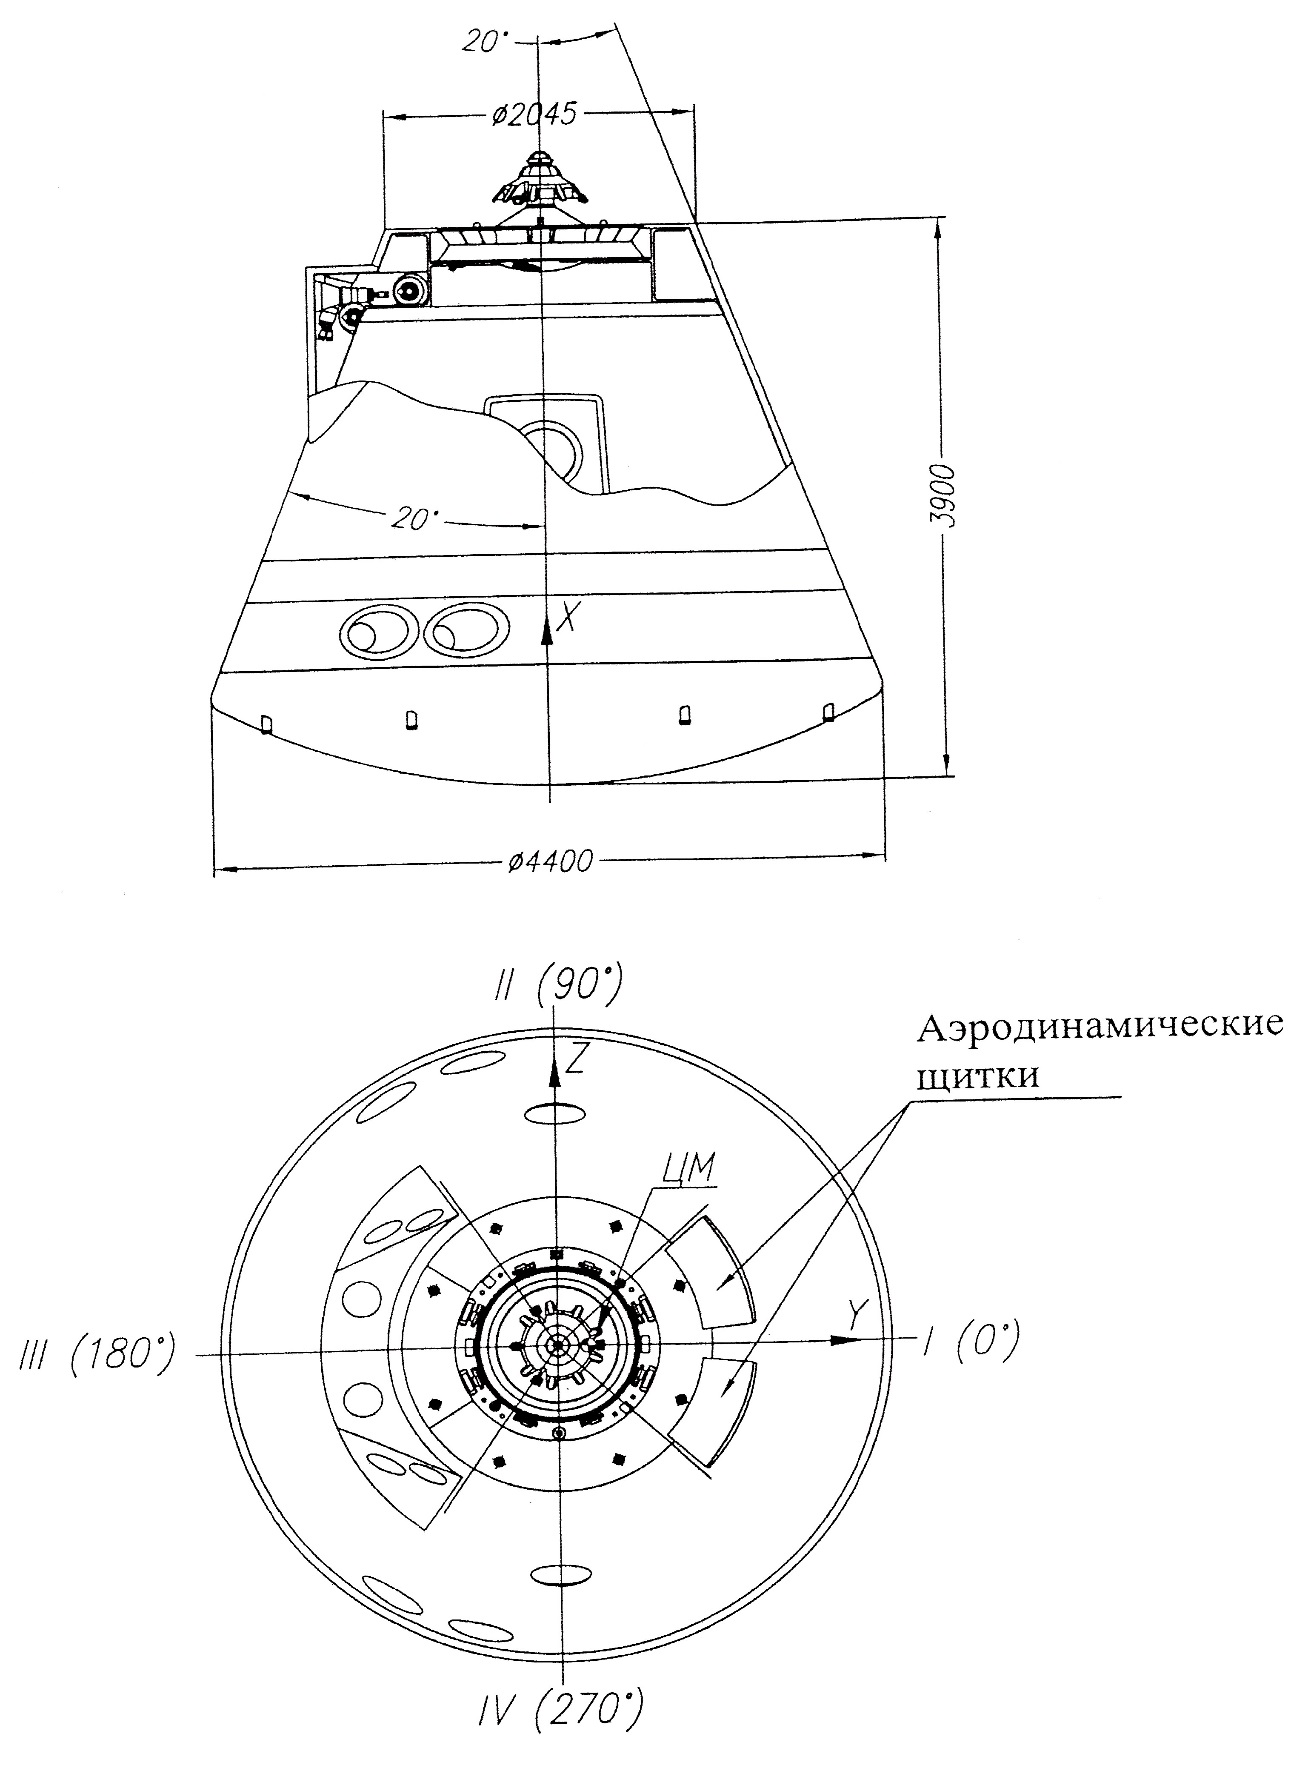
\includegraphics[scale=0.7]{images/va.jpg}
	\caption{Общий вид ВА}
	\label{fig:va_pic}
\end{figure}
\clearpage

\begin{figure}[h]
	\centering
	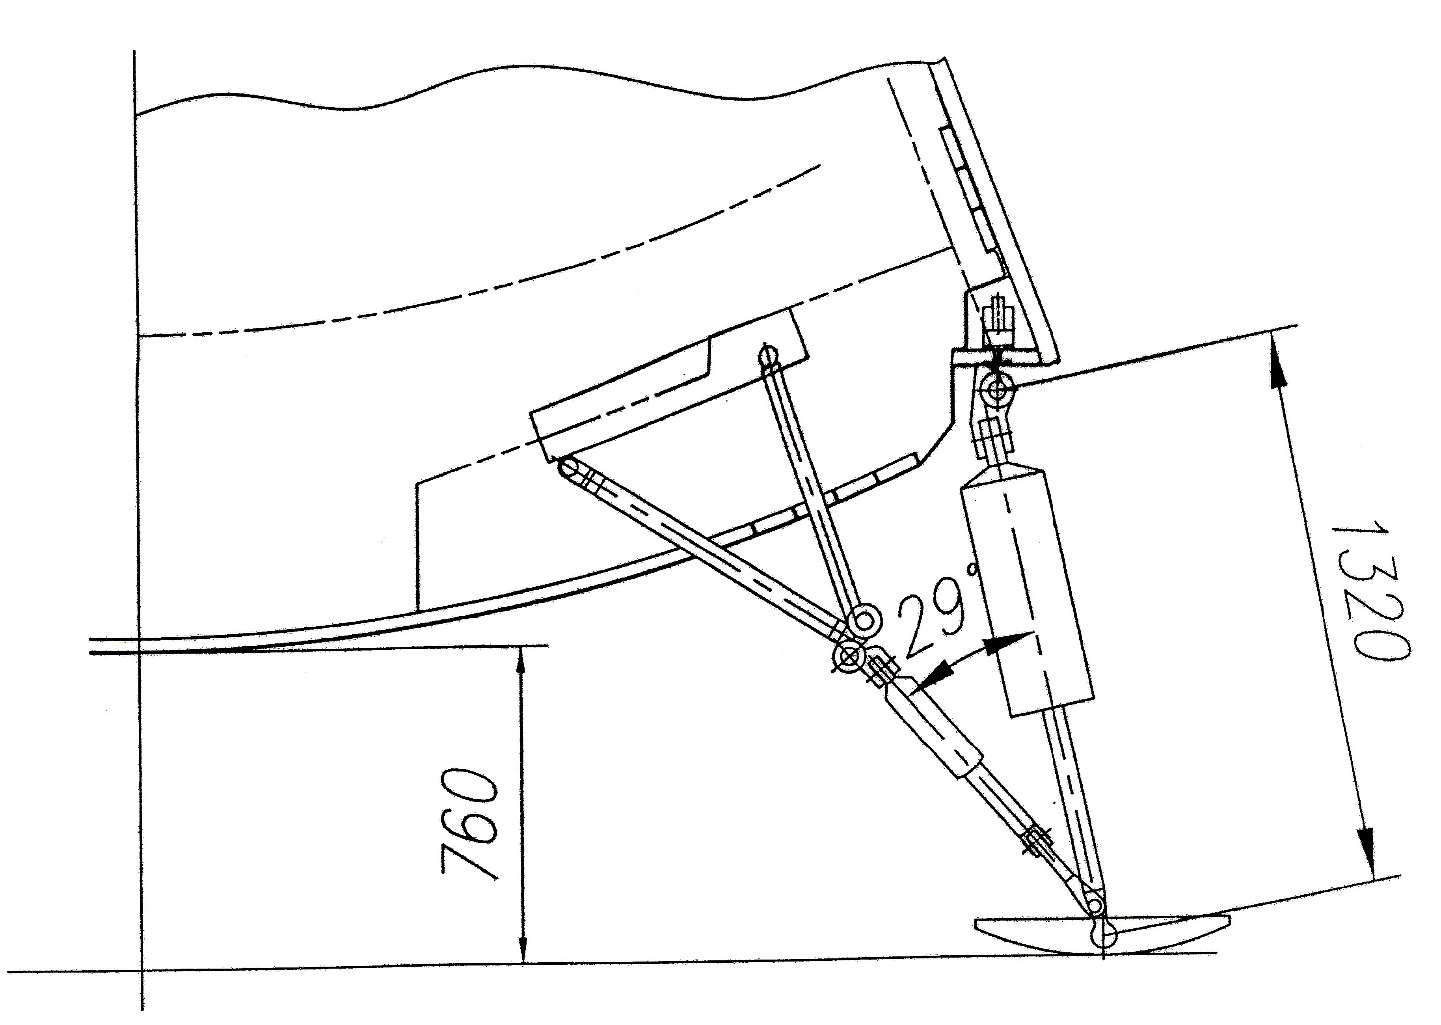
\includegraphics[scale=0.9]{images/posad_config.jpg}
	\caption{Посадочная конфигурация ВА с выпущенным посадочным устройством}
	\label{fig:posad_config}
\end{figure}
\clearpage

\subsection{Конструкция и принцип действия ПТДУ}
ПТДУ представляет собой РДТТ с регулируемой тягой по величине и направлению. На рисунке показана схема ПТДУ. Он состоит из:
\begin{itemize}
	\item двух корпусов типа "кокон"  с наполнителями ТРТ "Г-З"
	\item 16 односопловых управляющих блоков (СУБ)
	\item системы газоходов, газосвязывающего корпуса с наполнителями и СУБ
	\item двух пусковых двигателей 
	\item блока датчиков давления системы измерения давления
	\item рулевого привода (электромеханического или газогидравлического) 
\end{itemize}

Сопла всех СУБ снабжены собственными регуляторами расхода, управляемыми собственными рулевыми машинками. Расположение и маркировка органов управления соответствует рисунку 6.1.

ПТДУ многорежимна. Переход с режима на режим, а также стабилизация давления на любом режиме, обеспечивается изменением газоприхода от поверхности горения за счет изменения скорости горения наполнителя путем кратковременного изменения суммарной площади минимальных сечений сопел.

Создание управляющих сил по каналам тангажа и рыскания на каждом режиме обеспечивается за счет перераспределения расхода продуктов сгорания ТРТ между соплами путем изменения площади минимального сечения каждого сопла при сохранении постоянной суммарной площади минимальных сечений всех сопел:
\begin{equation}
\mu F_{\sum} = \sum_{j=1}^{16} \mu F_j \approx const
\end{equation}
где $\mu F_{\sum}$ - требуемая суммарная эффективная площадь минимальных сечений сопел на соответствующем режиме работы ПТДУ.

$\mu F_j$ - текущая эффективная площадь минимального сечения $j$-го сопла.

При необходимости должна быть обеспечена возможность отсечки тяги ПТДУ по команде СУ. При этом для прекращения горения наполнителей должно выполняться условие:
\begin{equation}
\mu F_{\sum} = \sum_{j=1}^{16} \mu F_j^{max}
\end{equation}
где $\mu F_j^{max}$ - максимальная эффективная площадь минимального сечения $j$ - го сопла.

В случае отказа одного из СУБ или отказа ПМ площадь минимального сечения этого СУБ при дальнешей работе ПТДУ должна оставаться постоянной, при это должна выполняться заданная циклограмма суммарной тяги $R_{\sum}$  и управление остальными СУБ в заданном диапазоне $R$.
\begin{figure}[h]
	\centering
	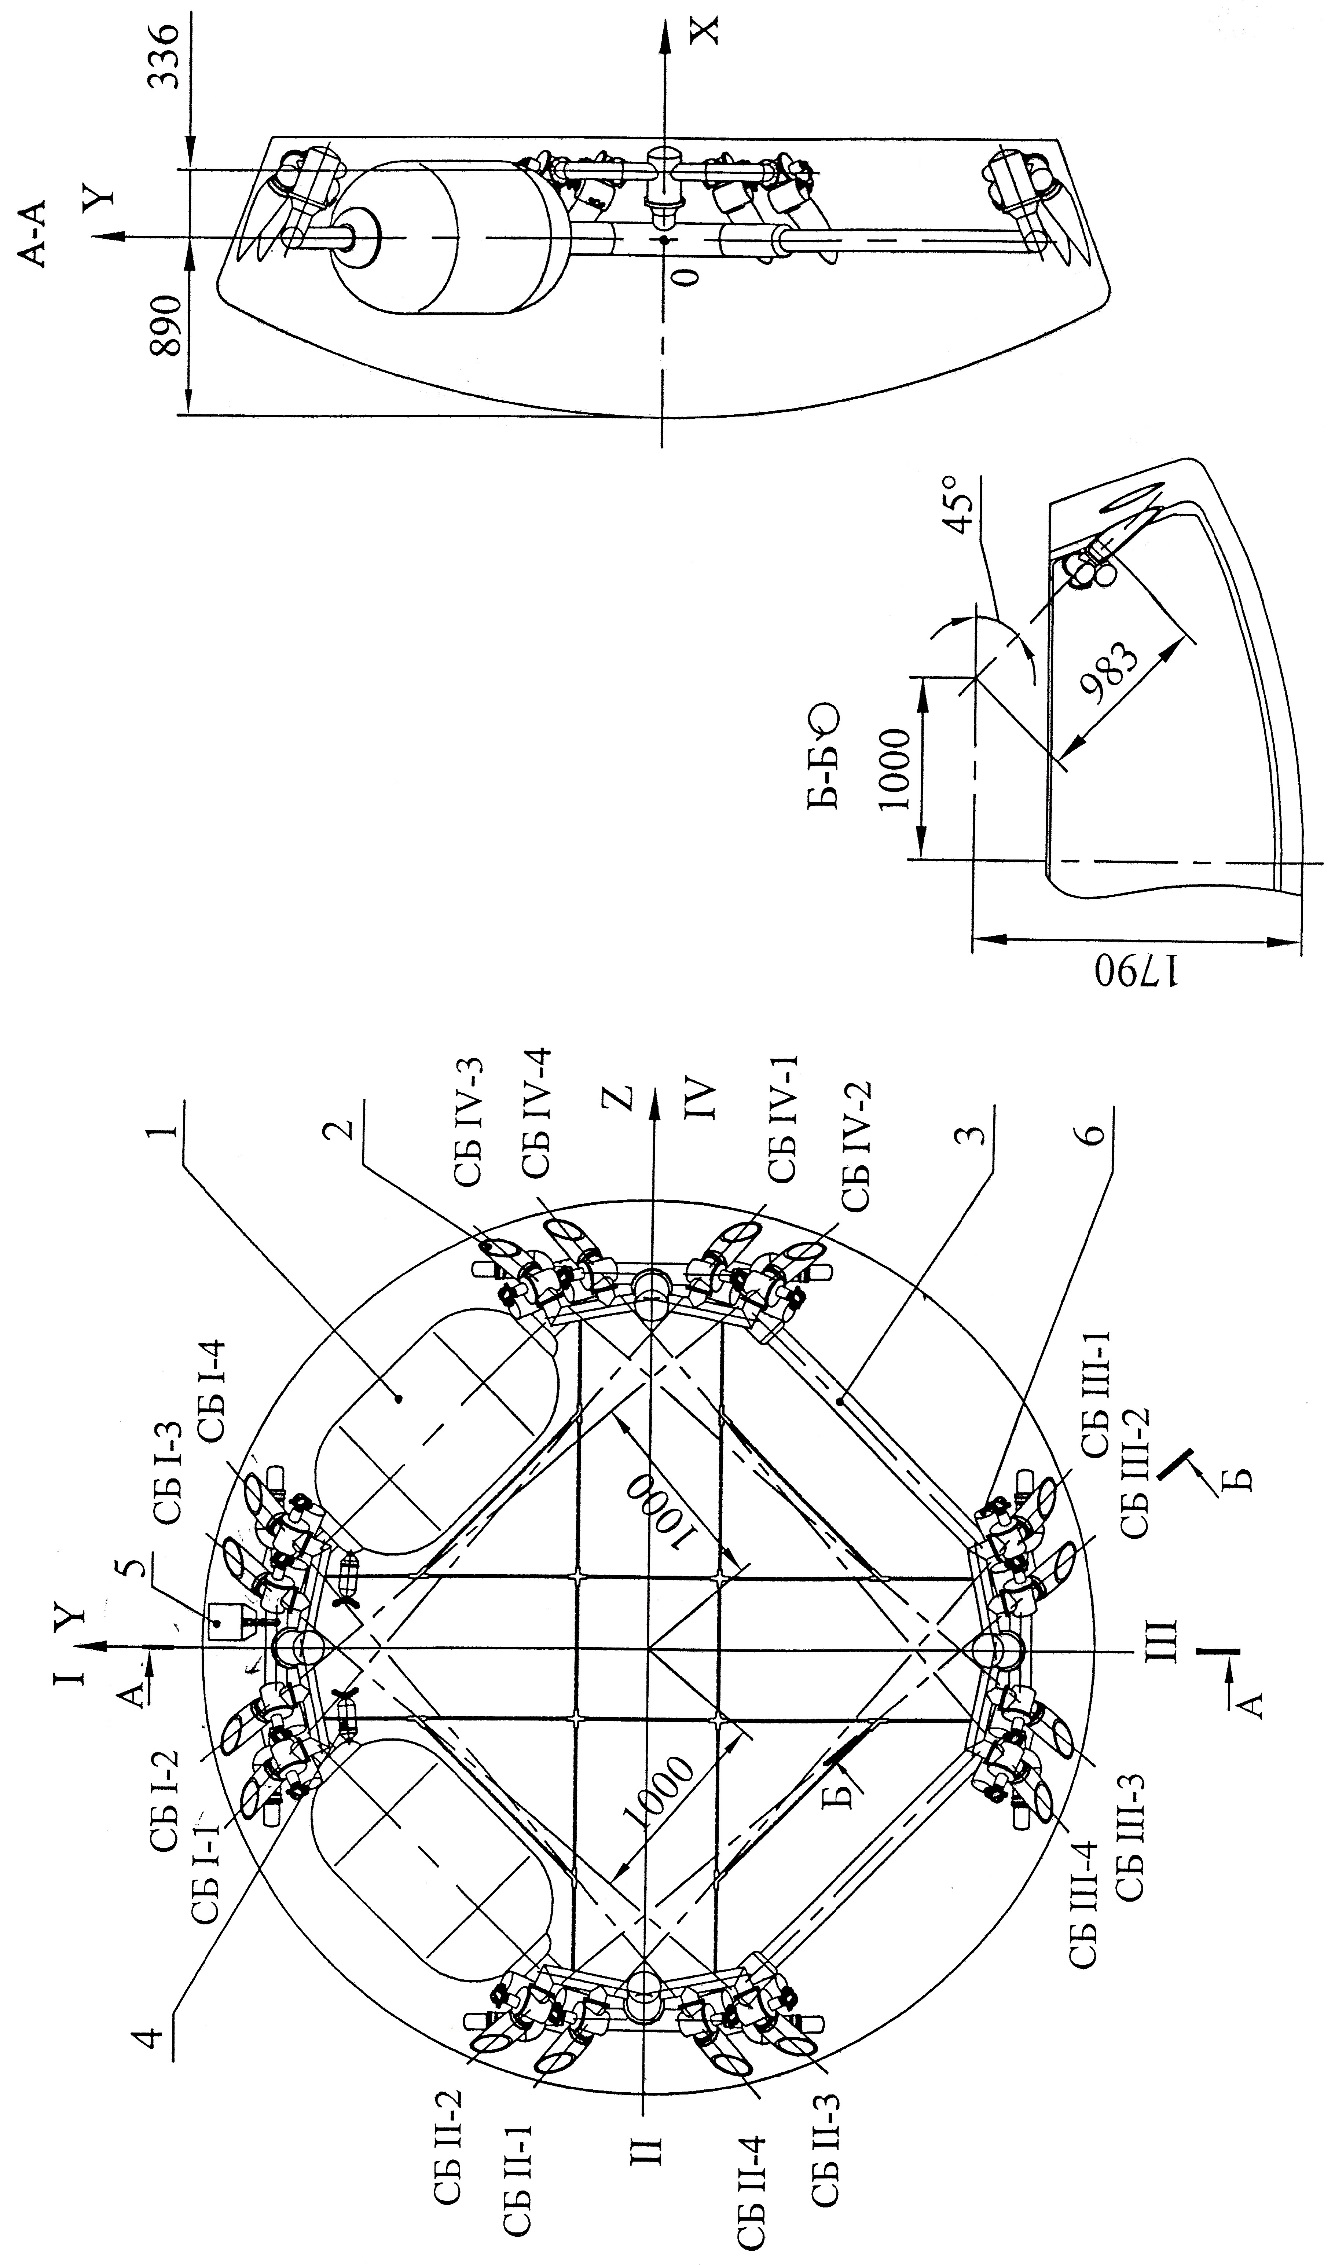
\includegraphics[scale=0.3]{images/scheme_ptdu.jpg}
	\caption{Схема ПТДУ}
	\label{fig:scheme_ptdu}
\end{figure}
\clearpage

\subsection{Характеристики органов управления}

\begin{figure}[h]
	\centering
	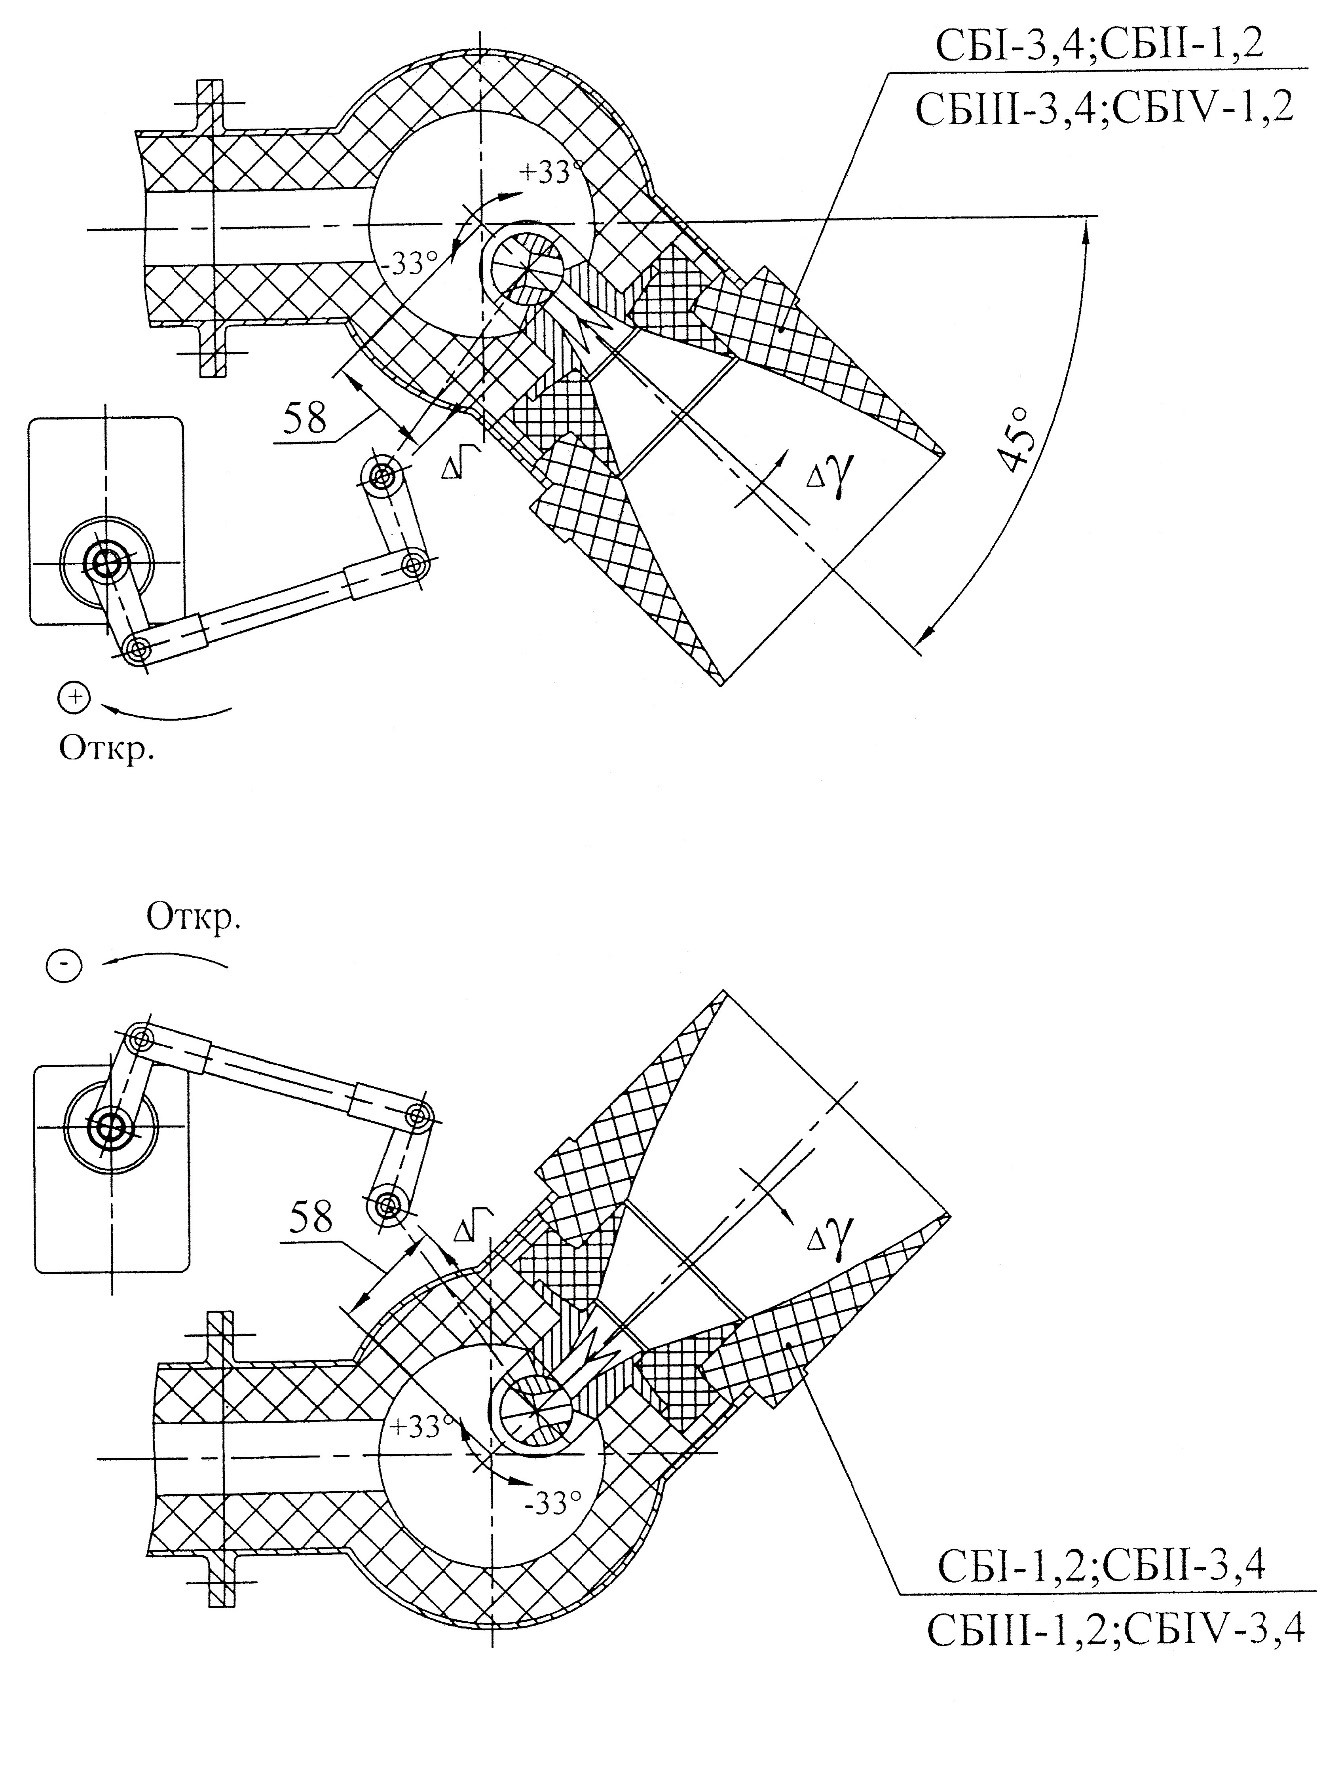
\includegraphics[scale=0.5]{images/scheme_subrp.jpg}
	\caption{Кинематическая схема СУБ с РП}
	\label{fig:scheme_subrp}
\end{figure}

Зависимость эффективной площади минимального сечения единичного сопла СУБ ($\mu F_j$) от угла поворота вала РМ ($\delta_j$ ) представлена на рисунке ~(\ref{fig:effect_nozzle})

\begin{figure}[h]
	\centering
	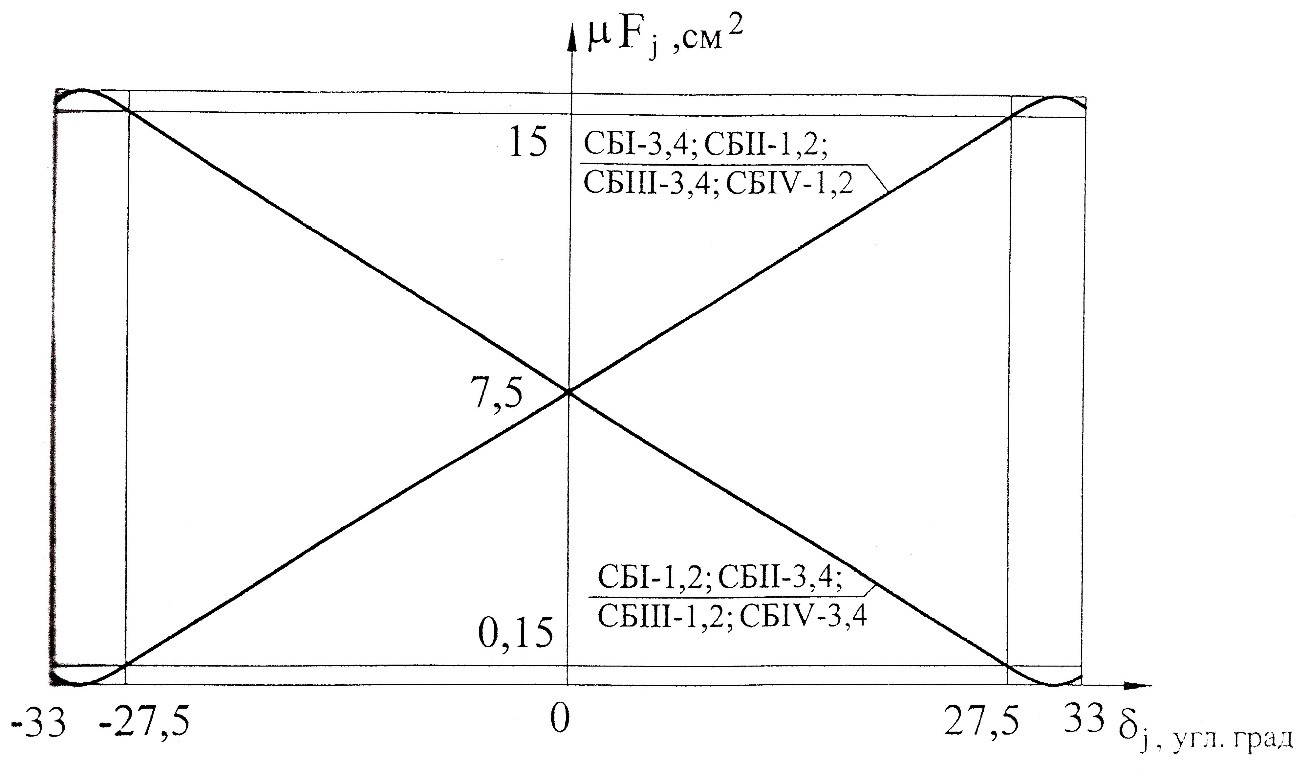
\includegraphics[scale=0.5]{images/effect_nozzle.jpg}
	\caption{Зависимость эффективной площади сечения единичного сопла ($\mu F_j$) от угла поворота вала РМ ($\delta_j$)}
	\label{fig:effect_nozzle}
\end{figure}

При работе ПТДУ используется только линейный участок зависимости $\mu F_j (\delta_j)$.

На участке от $-27.5^{\circ}$ до $27.5^{\circ}$ для данной расходной характеристики допускается линейная аппроксимация:
\begin{equation}
	\label{eq:ur_lin_approxim}
	\delta_j = 3.667 \cdot \mu F_j - 27.5
\end{equation}

Систематическое линейное и угловое отклонение вектора тяги в единичном сопле в зависимости от угла поворота РМ от геометрической оси сопла за счет прямоугольной формы площади минимального сечения регулятора сопла приведено на ~(\ref{fig:effect_nozzle}).

Отклонение происходит в плоскости, проходящей через геометрическую ось сопла перпендикулярно продольной оси корпуса СУБ.

Случайное отклонение вектора тяги от номинального положения геометрической оси сопла в плоскости минимального сечения составляет: линейное $1.5$ мм, угловое $1.5^{\circ}$.

\begin{figure}[h]
	\centering
	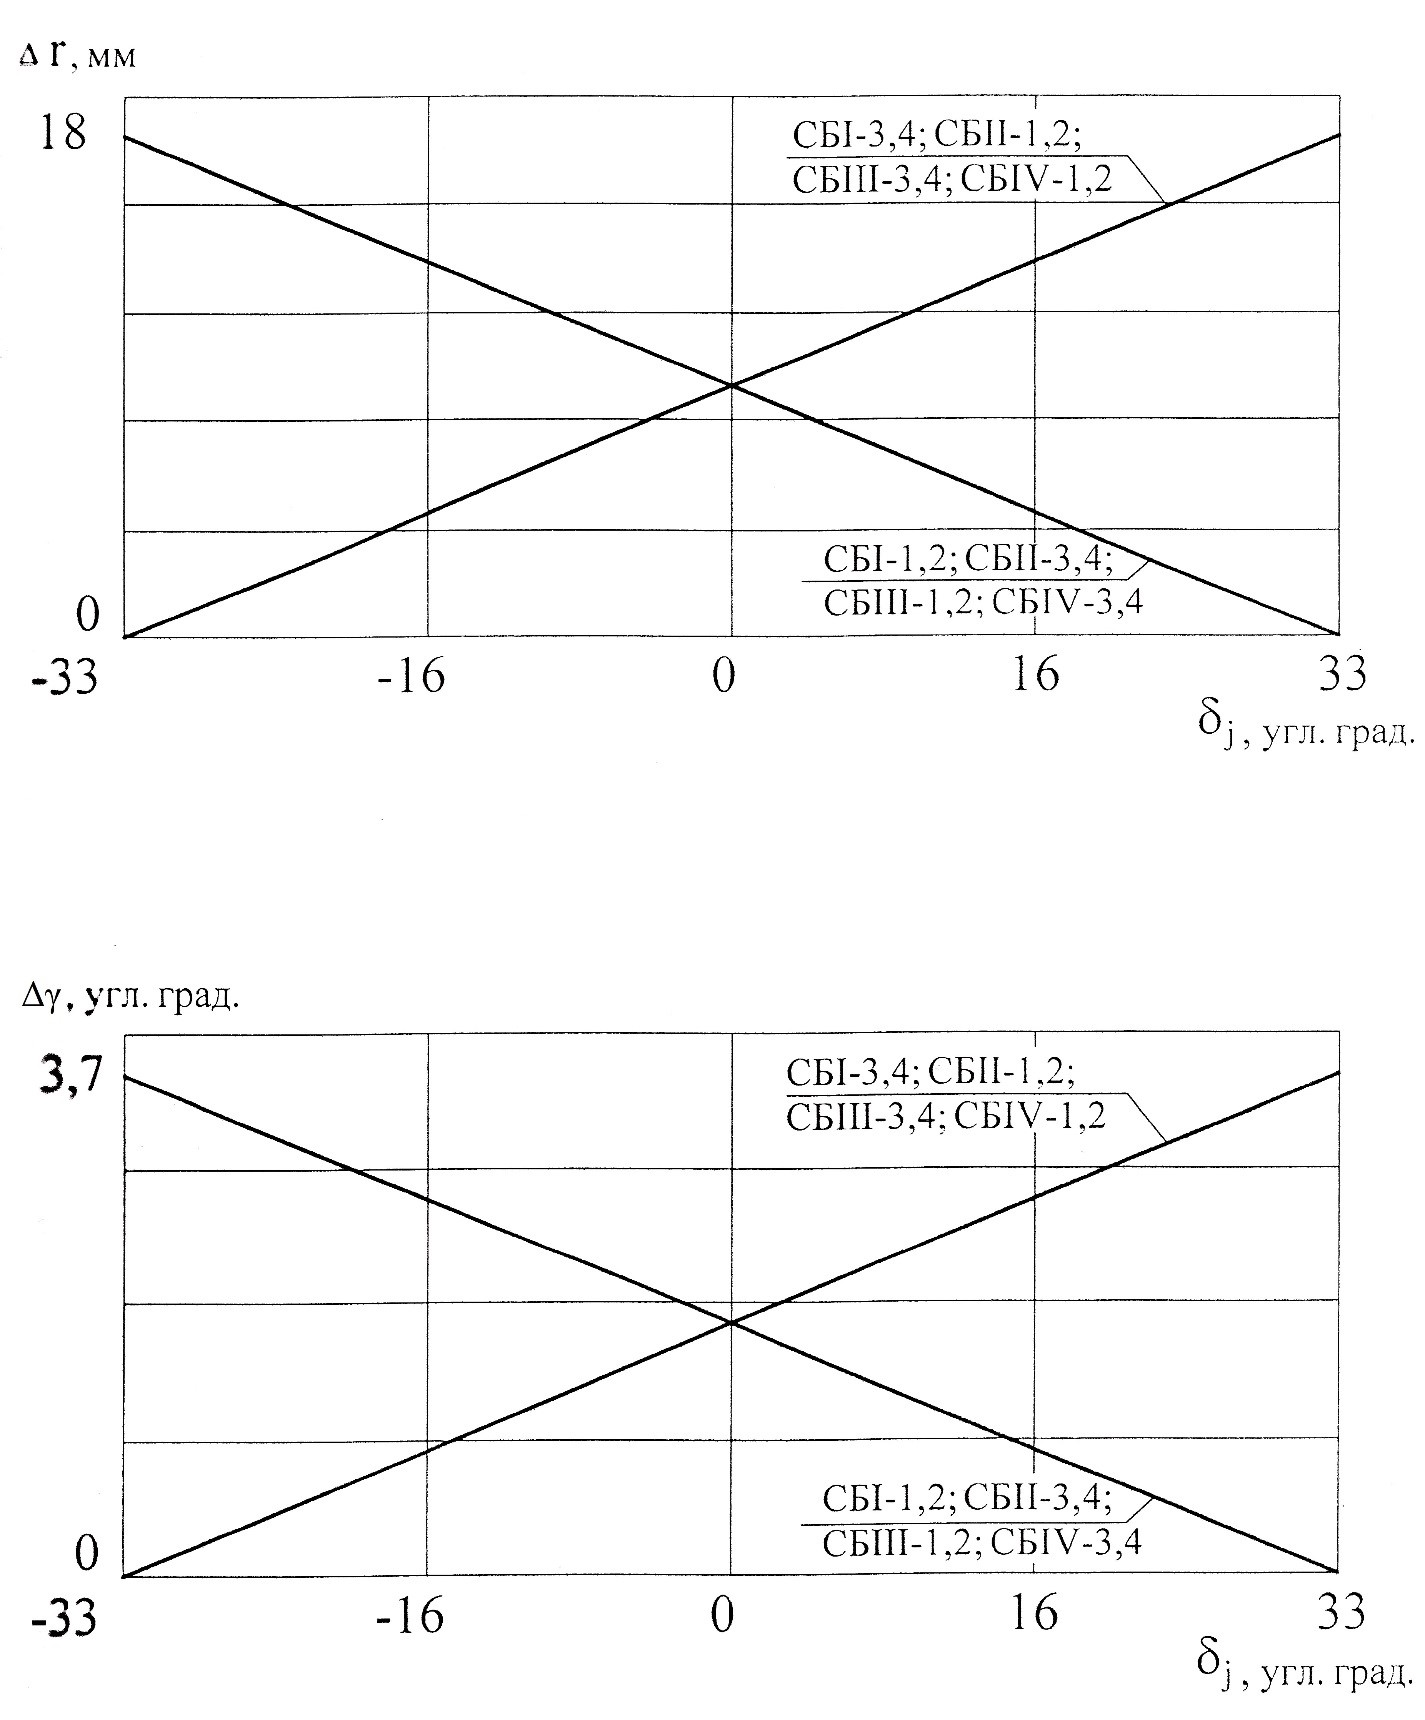
\includegraphics[scale=0.5]{images/linear_vect_draft.jpg}
	\caption{Линейное ($\Delta r$) и угловое ($\Delta \gamma$) отклонение линии действия вектора тяги от геометрической оси сопла в зависимости от угла поворота вала РМ}
	\label{fig:lin_angle_otklonenie}
\end{figure}

\clearpage

\subsection{Требования к СУ}
Исходными данными на разработку технических предложений по алгоритмам СУ, СУ ПТДУ для управления на участке посадки возвращаемого аппарата определены следующие положения:
\begin{itemize}
	\item Начальные условия при запуске ПТДУ:
	\begin{itemize}
		\item угол наклона траектории $-70^{\circ} \div -90^{\circ}$
		\item скорость $80 \div 120 \frac{\text{м}}{\text{с}}$
		\item угол атаки $8^{\circ} \div 20^{\circ} $
		\item угловые скорости до $\pm 50$ угл. град/с по трем углам одновременно
		\item высота $700 \div 1200$ м.
	\end{itemize}
	\item Условия окончания:
	\begin{itemize}
		\item на высоте ~ $20$ м начинается участок вертикального движения, который завершается касанием. Скорость во время касания $2 \div 3 \frac{\text{м}}{\text{с}}$
	\end{itemize}
	\item суммарный импульс тяги:
	$$\int \limits_{0}^T R(r) dt = 280 \ \text{Тс} \cdot c$$
\end{itemize}
\clearpage
	
	%	Алгоритм определения момента включения ПТДУ
	%	Алгоритм определения момента включения ПТДУ
\section{Алгоритм определения момента включения ПТДУ}
Исходя из независимости движений в ортогональных направлениях и приоритете вертикального канала в процессе управления, выбор момента включения ДУ определяется высотой, скоростью движения аппарата и необходимостью обеспечения наиболее предпочтительного режима работы ПТДУ.

Предпочтительным режимом является работа в середине линейного диапазона регулирования тяги, так как при действии возмущений такой режим создает наилучшие условия для управления.

В связи с тем, что аппарат на момент включения ПТДУ движется практически с установившейся скоростью, суммарная потенциальная и кинетическая энергия, которую необходимо рассеять с помощью ПТДУ, убывает при снижении аппарата:

\begin{equation}
E(h) = \frac{mv^2}{2} + mgh
\end{equation}
где $v \ \approx const$

Принимая равенство совершаемой двигателем работы и энергии аппарата, погашаемой на участке спуска при величине тяги двигателя, соответствующей середине диапазона регулирования $E = R_{cp} \eta_0$, получаем высоту включения ПТДУ:

\begin{equation}
\eta_0 = \frac{m v^2}{2} \cdot \frac{1}{R_{cp} + C_x \rho S_m \frac{v^2_\eta}{6} - mg}
\end{equation}
здесь $R_{cp} = 12$Тс.

Этот функционал может вычисляться на борту и при возможном разбросе начальной скорости $v_{\eta_0}$ в пределах $80 \div 120 \frac{\text{м}}{\text{с}}$, высота включения ПТДУ лежит в пределах $\eta_0 = 400 \div 800\text{м}$. 
Предполагая, что в вертикальном канале реализуется движение с постоянным замедлением, т. е. $\Dot{V}_\eta = const$, получаем интегралы движения:
\begin{equation}
\eta = \eta_0 - V_\eta \cdot t + \frac{\Dot{V}_\eta \cdot t^2}{2}
\label{eq:int-eq}
\end{equation}
\begin{equation}
V_\eta = -V_{\eta_0} + \Dot{V}_\eta \cdot t
\end{equation}
откуда
\begin{equation}
\Dot{V}_\eta = \frac{V^2_{\eta_0}}{2 \eta_0}
\label{eq:usk_v_eta}
\end{equation}
\begin{equation}
T = -\frac{V_{\eta_0}}{\Dot{V}_\eta}
\end{equation}

Среднее значение вертикального ускорения, обеспечивающего затормаживание на заданной высоте $\Dot{v}_\eta \approx 12 \div 20 \frac{\text{м}}{\text{с}^2}$, и время торможения $T \approx 8 -10 $с. При этом минимальный суммарный импульс тяги, расходуемый на затормаживание аппарата равен $\approx 150 \text{Тс} \cdot \text{с}$. На участке вертикального спуска расходуется еще $\approx 70 \div 80 \text{Тс} \cdot \text{с}$.

Минимальная высота включения ПТДУ, при которой еще возможно
погасить энергию аппарата $h_0 \approx 400 \text{м}$, время торможения $\approx 7 \text{c}$, тяга $R_{max} = 22 \text{Тс}$. При этом перемещения в горизонтальной плоскости исключаются. Весь импульс при этом сбрасывается в вертикальном канале управления.
\clearpage
	
	%	Математическая модель движения ЦМ ВА
	%	Математическая модель движения ЦМ ВА
\section{Математическая модель движения ЦМ ВА}
Модель движения ЦМ запишем в следующем виде:
\begin{equation}
	\left\{ \begin{matrix}
			\dot{W}_{X1} = \frac{F_{X1}}{m} \\
			\dot{W}_{Y1} = \frac{F_{Y1}}{m} \\
			\dot{W}_{Z1} = \frac{F_{Z1}}{m} \\
		\end{matrix} \right. ,
\end{equation}
где $\dot{W}_{X1}$, $\dot{W}_{Y1}$, $\dot{W}_{z1}$ - проекции кажущегося ускорения на оси связанной системы координат, $F_{X1}$, $F_{Y1}$, $F_{Z1}$ - проекции сил действующих на ВА, $m$ - масса ВА.

\begin{equation}
	\begin{gathered}
		F_{X1} = X - R_{\sum}, \\ 
		F_{Y1} = F_{\text{упр}Y1} + Y, \\
		F_{Z1} = F_{\text{упр}Z1} + Z,
	\end{gathered}
\end{equation}
где $R_{\sum}$ - суммарная сила тяги действующая по оси $OX_1$ связанной системы координат, $F_{\text{упр}Y1}$ - управляющая сила действующая по оси $OY_1$ связанной системы координат, $F_{\text{упр}Z1}$ - управляющая сила действующая по оси $OZ_1$ связанной системы координат, $X$ - продольная составляющая аэродинамической силы, $Y$ - нормальная составляющая аэродинамической силы, $Z$ - поперечная составляющая аэродинамической силы.
\clearpage

\subsection{Расчет управляющих сил}

На ЛА во время полета также действуют управляющие силы и моменты, которые создаются с помощью СУБ

%рисунок направление тяги
Угол наклона сопел равен $\alpha_c = 5.73^{\circ}$ показан на рисунке , максимальная суммарная тяга равна $$R_{max}^{\sum} = 22 \text{Тс}$$

Максимальная тяга $i$ - го сопла $$R_{\max i} = 2.75 \text{Тс}$$

Минимальная суммарная тяга $$R^{\sum}_{\min} = 8 \text{Тс}$$

Минимальная тяга $i$ - го сопла $$R_{\min i} = 1 \text{Тс}$$

\clearpage

\subsection{Расчет аэродинамических сил}
При полете ЛА в атмосфере на них действует сопротивление воздуха, называемое аэродинамическим.

Аэродинамическая сила $R_A$ складывается из сил давления воздуха, направленных по нормалям к поверхности ЛА, и сил трения воздуха касательных к ней. 

Для определения $R_{A}$ используют формулу:
\begin{equation}
	R_{A} = C_{R} \cdot q \cdot S, 
\end{equation}
где $q = \frac{\rho \cdot V^2}{2}$ - скоростной напор набегающего невозмущенного потока, $V$ - скорость набегающего потока, $\rho$ - плотность атмосферы, $S_\text{м}$ - характерная площадь ракеты, $M$ - число маха ракеты, $C_R$ - безразмерный аэродинамический коэффициент, зависящий от формы ракеты.

Запишем формулу для нахождения аэродинамической силы в плоскости $O Y_1 Z_1$:
\begin{equation}
	R_{Y_1 Z_1} = C_{Y1} (\alpha^*, M) \cdot q \cdot S_M
\end{equation}

Продольную составляющую аэродинамической силы запишем следующим образом: 
\begin{equation}
	X = C_{X_1} \cdot q \cdot S_M
\end{equation}

Нормальная составляющая аэродинамической силы:
\begin{equation}
	Y = R_{Y_1 Z_1} \cdot cos \varphi
\end{equation}

Поперечная составляющая аэродинамической силы:
\begin{equation}
	Z = -R_{Y_1 Z_1} sin \varphi
\end{equation}



\clearpage
	
	%	Общая постановка задачи синтеза СУ ПТДУ
	%	Общая постановка задачи синтеза СУ ПТДУ
\section{Общая постановка задачи синтеза СУ ПТДУ}
Исходя из требований ТЗ, при н. у. которые были определены ранее решенной задачей определения момента включения ПТДУ, требуется переместить объект из одной из возможных точек области н. у. в заданную точку пространства (точка зависания) за заданное время. В связи с тем, что органами управления являются не поворачиваемые сопла, т. о. сама задача определяется движением ЦМ и угловым движением. В связи с компоновкой сопловых блоков ВА эти задачи взаимосвязаны. Для того чтобы упростить задачу на данном этапе синтеза будем считать что есть приведенные моменты и приведенные силы. Распределения сил и моментов по соплам это задача следующего этапа. Чтобы синтез управления упростить мы декомпозируем систему на две независимые подсистемы: управления ЦМ и Управления угловым положением на основе разделения движений. Считаем, что динамика требуемой угловой ориентации на порядок быстрее чем движения ЦМ.

При этом каждой из этих подсистем управления выдвигаются свои требования по качеству:
\begin{enumerate}
	\item Время переходного процесса
	\item Осутствие перерегулирования
	\item Точность вывода в точку при вариации н. у. в области, которая ранее была определена алгоритмом включения ПТДУ
\end{enumerate}
\newpage

\subsection{Постановка задачи управления ЦМ}

Цель управления: 
\begin{equation}
|| x(t) - x_{*}(t) || \leq \Delta_x, \  \forall t \geq \hat{t}
\label{eq:ur_target_control}
\end{equation}
где $x(t) = (\xi \ \dot{\xi} \ \eta\  \dot{\eta} \ \zeta \ \dot{\zeta})^T$ - вектор состояния объекта управления относительно центра масс, $x_{*}(t)$ - желаемая траектория спускаемого аппарата с заданными показателями качества.

Это была общая постановка задачи управления. Для того чтобы решить данную задачу мне нужно прежде всего сформировать желаемую траекторию и стабилизироваться относительно 
её.

Таким образом, задача распадается на две подзадачи:
\begin{enumerate}
	\item Синтез желаемой кинематической траектории с учетом желаемой динамики движения по данной траектории.
	\item Стабилизация ЦМ ВА относительно желаемой траектории (задача слежения)
\end{enumerate}
\clearpage
	
	%	Синтез желаемой кинематической траектории
	%	Синтез желаемой кинематической траектории
\section{Алгоритм наведения}

Мы имеем начальные условия и конечные координаты траектории на момент времени T. Кинематическая функция должна быть гладкой функцией хотя бы второго порядка.

Будем искать решение кинематической траектории в виде многочлена на единице меньше, чем количество краевых условий. Это связано с тем, что у многочлена степени $n$ в общем случае имеется $(n + 1)$ параметров, которые подлежат выбору. 

Краевыми условиями являются начальные и конечные координаты, скорости и ускорения. Т.о. в качестве функций описывающих траектории движения выберем полиномы пятого порядка:
\begin{equation}
	\alpha(t) = \alpha_0 + \alpha_1 t + \alpha_2 t^2 + \alpha_3 t^3 + \alpha_3 t^4 + \alpha_5 t^5 
	\label{eq:ur_traectorii}
\end{equation}

\begin{equation}
	\Dot{\alpha}(t) = \alpha_1 + \alpha_2 t + \alpha_3 t^2 + \alpha_3 t^3 + \alpha_5 t^4 
	\label{eq:ur_velocity}
\end{equation}

\begin{equation}
	\Ddot{\alpha}(t) = 2 \alpha_2 + 6 \alpha_3 t + 12 \alpha_4 t^2 + 20 \alpha_5 t^3
\end{equation}
Где $\alpha(t)$ любая из координат $\xi(t)$, $\eta(t)$, $\zeta(t)$, $t$ - время, на котором действуют коэффициенты $a_0-a_5$. 

Задаваясь начальными и конечными значениями координат $\alpha (0)$, $\dot{\alpha} (0)$, $\ddot{\alpha} (0)$, и $\alpha (T)$, $\dot{\alpha} (T)$, $\ddot{\alpha} (T)$ получаем три тройки уравнений относительно $a_{3 \xi}$, $a_{3 \eta}$ , $a_{3 \zeta}$, $a_{4 \xi}$, $a_{4 \eta}$ , $a_{4 \zeta}$, $a_{5 \xi}$, $a_{5 \eta}$ , $a_{5 \zeta}$ добавляя к ним коэффициенты $a_{0 \xi}$, $a_{0 \eta}$ , $a_{0 \zeta}$, $a_{1 \xi}$, $a_{1 \eta}$ , $a_{1 \zeta}$, $a_{2 \xi}$, $a_{2 \eta}$ , $a_{2 \zeta}$, которые определяются начальными условиями, имеем следующее решение для определения многочленов пятого порядка:
\begin{equation}
	\begin{gathered}
		a_0 = \alpha (0), \\
		a_1 = \dot{\alpha} (0) \\
		a_2 = \ddot{\alpha} (0) \\
		a_3 = \frac{10 \cdot ( a(T) - a(0) ) }{T^3} - \frac{4 \cdot \dot{a}(T) + 6 * \dot{a}(0) ) }{T^2} +  \frac{ \ddot{a}(T) - 3 \cdot \ddot{a}(0) }{2 \cdot T}\\
		a_4 = \frac{-15 \cdot ( a(T) - a(0) ) }{T^4} + \frac{7 \cdot \dot{a}(T) - 8 * \dot{a}(0) ) }{T^3} +  \frac{ 1.5 \cdot \ddot{a}(T) -  \ddot{a}(0) }{T^3} \\
		a_5 = \frac{6 \cdot ( a(T) - a(0) ) }{T^5} + \frac{3 \cdot \dot{a}(T) - \dot{a}(0) ) }{T^4} +  \frac{\ddot{a}(T) -\ddot{a}(0) }{T^3} \\
	\end{gathered}
\end{equation}
$T$ - время, оставшееся до окончания процесса, начальное значение которого определяется в момента запуска ПТДУ.
\clearpage

\subsection{Формирование вектора требуемой ориентации ВА}
Требуемая ориентация ветора тяги находится из компонент вектора требуемого кажущегося ускорения в виде соответствующих направляющих косинусов
\begin{equation}
	\overline{e}^R = (e^{R}_\xi, e^{R}_\eta, e^{R}_\zeta)
\end{equation}

\begin{equation}
	\begin{gathered}
		\dot{W}^\text{ТР}_\xi = \dot{V}_\xi, \\
		\dot{W}^\text{ТР}_\eta = \dot{V}_\eta + g, \\
		\dot{W}^\text{ТР}_\zeta = \dot{V}_\zeta,
	\end{gathered}
\end{equation}

Рассчитываем требуемое кажущиеся ускорение ЛА
\begin{equation}
	\dot{W}_\text{ТР} = \sqrt{ \dot{W}^{\text{ТР}^2}_\xi + \dot{W}^{\text{ТР}^2}_\eta +\dot{W}^{\text{ТР}^2}_\zeta }
\end{equation}

Так как требуемое направление оси $X$ противоположно направлению тяги, выражения принимают следующий вид:
\begin{equation}
	\begin{gathered}
		e^R_\xi = - \frac{\dot{W}^\text{ТР}_\xi}{\dot{W}_\text{ТР}}, \\
		e^R_\eta = - \frac{\dot{W}^\text{ТР}_\eta}{\dot{W}_\text{ТР}}, \\
		e^R_\zeta = - \frac{\dot{W}^\text{ТР}_\zeta}{\dot{W}_\text{ТР}} \\
	\end{gathered}
\end{equation}
\clearpage

	
	%	Синтез алгоритмов стабилизации
	%	Синтез алгоритмов стабилизации
\section{Синтез алгоритмов стабилизации}

\subsection{Метод модального управления}
Модальное управление - это методы формирования цепей обратных связей, придающих замкнутой системе заранее выбранное расположение корней характеристического уравнения.

Структура модального регулятора задается всегда одинаковой и представляет собой обратную связь по всем переменным состояния. Регулятор линейно преобразует поступившие сигналы, т.е. усиливает и суммирует эти сигналы $x_i$ и выдает в качестве выходы их линейную комбинацию.

Это управление применяется, когда все составляющие вектора состояния объекта управления доступны непосредственному измерению (полная управляемость). 
\begin{equation}
\Dot{x} = A x + B u
\label{eq:main_eq_modal_control}
\end{equation}

Для получения желаемого быстродействия и характеристического уравнения системы введем линейную обратную связь по переменным состояния в соответствии с уравнением
\begin{equation}
u = v - Kx,
\label{eq:eq_control}
\end{equation}

где $v$ - новое обозначение вектора входных воздействий, $u$ - вектор управляющих воздействий с выхода регулятора, $K$ - матрица обратной связи.

$K$ - является матрицей -  строкой, элементы которой - есть коэффициенты обратных связей по всем составляющим вектора $x$.
$$K = \left[ K_1 K_2 ... K_n \right]$$.

Структурная схема исходной системы с обратной связью по переменным состояния приведена на рис.~(\ref{fig:struct_scheme_feedback_variable_sost})

\begin{figure}[h]
	\centering
	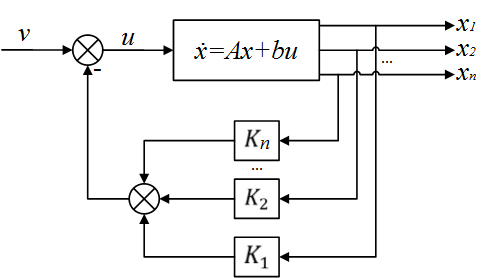
\includegraphics[scale=0.6]{images/struct_scheme_feedback_variable_sost.png}
	\caption{Структурная схема системы с обратной связью по переменным состояния}
	\label{fig:struct_scheme_feedback_variable_sost}
\end{figure}



Задача распределения корней характеристического уравнения замкнутой системы желаемым образом обеспечивает устойчивость заданной стабилизации и ее желаемую динамику быстродействия, перерегулирования и
т.п.

Рассмотрим линейный объект $\Dot{x} = Ax + Bu$ в форме пространства состояния.

В данном случае вектор $x$ включает в себя параметры угла и угловой скорости соответственно по каналам управления, $u$ - управление соответствующее приведенным моментам или силам действующее на летательный аппарат по рассматриваемому каналу.

Целью управления является 
$$||x(t) -  x^{*}(t)|| \rightarrow 0, \  t \rightarrow \infty, $$

где $x^{*}(t)$ - желаемая динамика замкнутой системы заданной эталонной модели.

Решение поставленной задачи методом модального управления находим в виде линейной обратной связи по составленному ОУ и заданному воздействию эталонной модели $\Dot{x}_{*}$.
\begin{equation}
\Dot{x}_{*} = A_{*} x_{*} + B_{*} u_{*},
\label{eq:ur_mod_contol_with_star}
\end{equation}
где 
$$A_{*} = \begin{pmatrix}
0 & 1 \\
- \alpha^{*}_0 & - \alpha^{*}_1 \end{pmatrix} \ B = \begin{pmatrix}0 \\ \alpha^{*}_0 \end{pmatrix}$$

Управляющее воздействие $u = K x + K_r y_{*}$.

Компоненты вектора $K = \begin{pmatrix} K_1 \\ K_2 \end{pmatrix}$ и скалярного коэффициента усиления $K_r$ определяется из соотношения:
\begin{equation}
BK = A_{*} - A
\label{eq:ur_mod_control_BK}
\end{equation}
\begin{equation}
BK_r = B
\label{eq:ur_mod_control_BKr}
\end{equation}

Решение первого матричного уравнения существует если матрицы $A$ и $A^{*}$ согласованы по структуре, а ОУ является управляемым, то есть выполняется условие:
\begin{equation}
\label{eq:usl_upr}
rang \left( B | AB|...|A^n B\right) = n
\end{equation}

В рассматриваемом случае это условие соответствует выполнению следующих условий:

\begin{equation}
\label{eq:usl_this_1}
det \left( B|AB\right) \neq 0
\end{equation}

Уравнения для определения $K_r$ должно быть разрешенным относительно $K_r$ при структурной согласованности $B$ и $B^{*}$.

\clearpage

\subsection{Постановка задачи слежения по ЦМ}
Для того чтобы использовать вышеприведенный метод мы преобразуем исходную модель в форме пространства состояния с учетом того, что $u_{\xi}$, $u_{\eta}$, $u_{\zeta}$ - моменты по каналам.

\begin{equation}
\label{eq:norm_slej}
|| x_i(t) - x_i^{\text{эм}} (t) || \leq \overline{\Delta}_{xi}, \ \forall t \geq T_{*},
\end{equation}
где $x_i^{\text{эм}}$ - траектория эталонной модели заданной в виде:
\begin{equation}
\label{eq:ur_etalon_traektor}
\Dot{x}_i^{\text{эм}} = A_{*i} x_i^{\text{эм}} + B_{*i} r_{*i},
\end{equation}
где $x_1 = (\xi \dot{\xi})^T$, $x_2 = (\eta \dot{\eta})^T$, $x_3 = (\zeta \dot{\zeta})^T$, $i = \overline{1, 3}$, $i$ - номер канала, $u_i$ - управление.
$$u_1 = u_{\xi}, \  u_2 = u_{\eta}, \ u_3 = u_{\zeta}$$
$$r_{*1} = \xi_{*} (t), \ r_{*2} = \eta_{*} (t), \ r_{*3} = \zeta_{*} (t).$$

Приведенная выше формализация позволяет уйти от исходной системы к системе, описанной выше и использовать метод модального управления. 

Желаемое качество отработки задается спектром матрицы эталонной модели: $\lambda_{*j}(A_{*i}):Re \lambda_{*j} < 0$ (устойчивость), с заданым расположением корней.

Задаем расположение корней так, чтобы ближайший к мнимой оси полюс задавал быстродействие системы, если он вещественный, то будет апериодическое движение, если будет пара ближайших к мнимой  комплексно-сопряженных корней, то колебательное движение.

Исходя из того, что у нас система 2-го порядка выбирались 2 полюса так чтобы из требований времени второй полис был отнесен дальше от мнимой оси, чтобы его динамика не сильно сказывалась

Точность определеяем выбором параметром матрицы $B_{*}$ так, чтобы статическая ошибка была равна 1.
\clearpage

\subsection{Результаты моделирования переходных процессов}
\clearpage

\subsection{Результаты моделирования системы стабилизации ЦМ}
\clearpage
	
	%	Анализ технической реализуемости системы стабилизации ЦМ
	%	Анализ технической реализуемости
\section{Анализ технической реализуемости системы стабилизации ЦМ}

Для реализации вышеописанной системы управления нам понадобятся такие технические средства, которые позволили бы нам измерять положение, скорость, ускорение нашего аппарата в пространстве.
\clearpage

\subsection{Выбор датчиков}

Акселерометры предназначаются для измерения ускорений движущихся объектов и для преобразования этих ускорений в сигнал, используемый для определения параметров траектории  движения объекта или для целей автоматического управления этой траекторией. Акселерометры применяются для измерения линейных и угловых ускорений. В соответствии с этим они называются линейными акселерометрами или угловыми акселерометрами.

По назначению различают следующие акселерометры: для визуального контроля, для систем телеметрического контроля, для систем инерциальной навигации, для систем автоматического управления.

По исполнению акселерометры подразделяются на следующие две группы:\begin{itemize}
	\item пружинные, построенные по разомкнутой структурной схеме;
	\item компенсационные, построенные по замкнутой структурной схеме.
\end{itemize}

Компенсационные акселерометры, в свою очередь, делятся на акселерометры с позиционной обратной связью (акселерометры с «электрической пружиной»), со скоростной обратной связью (интегрирующие акселерометры) и с обратной связью по ускорению (акселерометры с двойным интегрированием). Акселерометры выполняют с непрерывным выходным сигналом или с дискретным.

Наиболее широкое применение акселерометры получили на летательных аппаратах. Как линейное, так и угловое ускорение движущегося в пространстве летательного аппарата можно в каждый момент времени разложить на три составляющие в системе координат, связанной с летательным аппаратом и ориентированной по его главным осям (осям симметрии).

Для получения полной информации о линейных и угловых ускорениях летательного аппарата необходимо иметь шесть акселерометров (три линейных и три угловых), измерительные оси которых ориентированы по главным осям летательного аппарата и каждый из которых измеряет соответствующий компонент линейного или углового ускорения.

В системах автоматического управления траекторией полета иногда используют не полную информацию, а лишь некоторую ее часть, например ограничиваются применением двух линейных акселерометров, измеряющих компоненты линейных ускорений по поперечным осям летательного аппарата.

При использовании акселерометров в системах инерциальной навигации применяют два линейных акселерометра, измерительные оси которых ориентированы по двум взаимно перпендикулярным направлениям, лежащим в горизонтальной плоскости, причем одно из направлений обычно совмещают с плоскостью географического меридиана. Возможны и другие способы ориентации измерительных осей акселерометров в зависимости от выбранной системы координат.
\clearpage

\subsection{Реализация на БЦВК}

Бортовой цифровой вычислительный комплекс получает информацию от датчиков и бортовых систем, обрабатывает ее в режиме разделения времени между задачами и выдает управляющие воздействия на исполнительные органы и бортовые системы. Для обеспечения работы в реальном масштабе времени каждые 32,8 мс прерывается работа процессора, что создает предпосылки для периодического возвращения к решению одних и тех же задач.

Облик и структуру БЦВК во многом определяет требование сохранения работоспособности и обеспечения безопасности экипажа при любых двух отказах. В состав БЦВК входят две идентичные по структуре и оборудованию вычислительные системы: центральная (ЦВС) и периферийная (ПВС), каждая из которых включает в себя четыре бортовые цифровые вычислительные машины, работающие синхронно по одинаковым программам, фактически резервирующие друг друга и представляющие четыре параллельных канала, на выходе каждого из которых имеется встроенная резервированная схема сравнения, контролирующая команды, выдаваемые абонентам из всех четырех БЦВМ. При отказе одной из БЦВМ схема сравнения блокирует ее выход и вычислительная система продолжает работать в составе трех каналов, при отказе второй БЦВМ ситуация повторяется: выход отказавшей БЦВМ блокируется и система продолжает работать в составе двух каналов.

Как известно, программная синхронизация четырех БЦВМ в реальном масштабе времени при любом сочетании допустимых отказов является чрезвычайно сложной и недостаточно надежной. В связи с этим в ЦВС и ПВС используется не программная, а аппаратная синхронизация, для чего в составе БЦВК имеется единый кварцевый генератор, подающий во все восемь БЦВМ единую сетку тактовых импульсов частотой 4 МГц и с периодом прерывания 32,8 мс. Поскольку задающий генератор также должен удовлетворять требованию "надежная работа при двух отказах", он имеет пять каналов резервирования, на выходе каждого из которых установлена схема голосования "три из пяти". Кроме того, в состав БЦВК входит накопитель на магнитной ленте (МЛ) емкостью 819200 32-разрядных слов для хранения программного обеспечения и загрузки его в оперативную память БЦВК в процессе полета.

В связи с тем, что нам нужно хранить и обрабатывать данные предполагается, что это будет происходить в бортовом цифровом вычислительном комплексе, при этом надо учитывать шаг дискретизации синтезируемых алгоритмов управления которые влияют на точность. Бортовая цифровая вычислительная техника — оборудование, входящее в единый комплекс и предназначенное для обеспечения сбора и обработки данных. В процессе работы бортовой цифровой вычислительный комплекс после сбора данных со всех систем и последующей обработки выдает управляющие воздействия на бортовые системы и исполнительные органы управления. Чтобы процесс шел в реальном времени, через определенные промежутки времени необходимо прерывать работу процессора для периодического возращения процессора к решению одних и тех же рабочих задач. Отличие БЦВМ от различных специализированных вычислителей и блоков обработки данных (которых в современном самолёте предостаточно) в том, что БЦВМ имеют общепринятую для компьютеров структуру: наличие оперативной и долговременной памяти, устройств ввода-вывода и т. д. Важной особенностью управления бортовыми системами является программное управление их резервированием. Сложная логика управления избыточностью требует проведения коммутации соответствующих схем и элементов строго по циклограммам управления, поэтому БЦВК не только анализирует числовые значения контрольных величин, но и задает и контролирует временные соотношения в ходе выполнения полетных задач. Предполагаем, что эта задача будет рассмотрена на следующем этапе разработки.
\clearpage
	
	%	Заключение
	%	Заключение
\anonsection{ЗАКЛЮЧЕНИЕ}
В данной работе была получена математическая модель движения центра масс возвращаемого аппарата (ВА), решена задача наведения, определена желаемая траектория, решена задача стабилизации по полученным желаемым траекториям, разработан алгоритм программного обеспечения  для проведенного математического моделирования подтверждающий работоспособность предлагаемых схем проведения углового движения с желаемой динамикой.

Разработана программа для моделирования движения ВА на языке программирования MatLab.

Полученные результаты удовлетворяют заданным погрешностям.
\clearpage
	
	%	Библиография
	%	Приложение
\end{document}
	